\documentclass[aspectratio=169,10pt]{beamer}

\usetheme{default}
\setbeamertemplate{navigation symbols}{}
\setbeamertemplate{footline}{%
  \hfill\usebeamerfont{page number in head/foot}\insertframenumber/\inserttotalframenumber\hspace{1.2em}\vspace{0.8em}
}
\setbeamertemplate{itemize item}{\raise0.2ex\hbox{\scriptsize$\blacktriangleright$}}
\setbeamertemplate{itemize subitem}{\raise0.2ex\hbox{\scriptsize$\triangleright$}}

\usepackage[T1]{fontenc}
\usepackage{lmodern}
\usepackage{amsmath,amssymb,booktabs,array}
\usepackage{graphicx}
\usepackage{tikz}
\usepackage[numbers,sort&compress]{natbib}
\providecommand{\doi}[1]{}
\usetikzlibrary{arrows.meta,positioning,calc}

\definecolor{ink}{RGB}{22,31,45}
\definecolor{slate}{RGB}{48,61,78}
\definecolor{muted}{RGB}{94,105,118}
\definecolor{rulegray}{RGB}{190,196,204}
\definecolor{deepblue}{RGB}{18,52,86}
\definecolor{wine}{RGB}{124,36,45}
\definecolor{forest}{RGB}{34,93,73}
\definecolor{paper}{RGB}{250,250,248}

\setbeamercolor{normal text}{fg=ink,bg=paper}
\setbeamercolor{frametitle}{fg=deepblue,bg=paper}
\setbeamercolor{title}{fg=deepblue}
\setbeamercolor{subtitle}{fg=slate}
\setbeamercolor{structure}{fg=deepblue}
\setbeamercolor{alerted text}{fg=wine}
\setbeamerfont{title}{series=\bfseries,size=\Large}
\setbeamerfont{frametitle}{series=\bfseries,size=\large}
\setbeamerfont{author}{size=\normalsize}
\setbeamerfont{date}{size=\small}
\setbeamerfont{jointwork}{size=\scriptsize}

\setlength{\parskip}{0.25em}
\renewcommand{\arraystretch}{1.18}

\newcommand{\E}{\mathbb{E}}
\newcommand{\Pbb}{\mathbb{P}}
\newcommand{\one}{\mathbf{1}}
\newcommand{\surv}{p_{\mathrm{surv}}}
\newcommand{\liq}{p_{\mathrm{liq}}}
\newcommand{\hf}{H}

\title[Optimal sizing under Kou jumps]{Optimal Sizing of Leveraged Crypto Long--Short Positions under Kou Jump-Diffusion via Killed Moments}
\author{Francis Liu}
\institute{Academic hour}
\date{30th June 2026}

\begin{document}

% ------------------------------------------------------------
\begin{frame}
  \vspace{1.0em}
  {\usebeamerfont{title}\usebeamercolor[fg]{title}\inserttitle\par}
  \vspace{1.2em}
  {\usebeamerfont{author}\insertauthor\par}
  \vspace{0.7em}
  {\usebeamerfont{jointwork}
    Joint work with Professor Daniel Pele, Department of Statistics and Econometrics,\\
    Bucharest University of Economic Studies\\
    Theodor Ginavar, PhD Candidate, MSCA Digital Finance\par}
  {\usebeamerfont{date}\insertinstitute\hspace{0.6em}|\hspace{0.6em}\insertdate\par}
  \vfill
  \begin{center}
    
\begin{tikzpicture}
      \draw[deepblue,very thick] (0,0) -- (10.8,0);
      \draw[wine,thick] (0,-0.12) -- (2.4,-0.12);
    \end{tikzpicture}
  \end{center}
  \vspace{0.8em}
  \large Method: survival probabilities and killed moments\quad Application: initial-buffer sizing
\end{frame}

% ------------------------------------------------------------
\begin{frame}{DeFi Lending Platforms}
  \small
  Aave / Compound: pooled lending
  \vspace{0.4em}

  \begin{itemize}
    \item \textbf{Mechanism} lenders supply pool assets; borrowers draw pooled liquidity
    \item \textbf{Accounting} no bilateral lender; protocol-level collateral and debt balances
    \item \textbf{Interest accrual} variable supply/borrow APRs; utilization-driven index growth
    \item \textbf{No fixed tenor} open-ended loans; no maturity date; no term structure contract
  \end{itemize}

  \vspace{0.25em}
  \textbf{Overcollateralization}
  \begin{itemize}
    \item Pseudonymous parties; no credit underwriting; no legal margin call
    \item Solvency and obligation enforcement entirely collateral-based
    \item No-arbitrage discipline through collateral constraint
    \item \textbf{Liquidator role} repay insolvent debt; seize collateral bonus; restore pool solvency
  \end{itemize}

\end{frame}

% ------------------------------------------------------------
\begin{frame}{Health Factor and Boundary}
  \small
  {\bf{Key mechanism variables}}
  \vspace{0.35em}

  State variables:
  \[
    V_{1,t}:=n_1S_{1,t}\quad\text{collateral value},
    \qquad
    V_{2,t}:=n_2S_{2,t}\quad\text{borrow/debt value}
  \]
  \vspace{0.25em}

  Loan-to-value* and liquidation threshold:
  \[
    \mathrm{LTV}_t:=\frac{V_{2,t}}{V_{1,t}},
    \qquad
    b=\mathrm{threshold\ LTV}
  \]
  Aave origination LTV $<$ threshold LTV $b$; initial buffer by design
  \vspace{0.25em}

  Health factor:
  \[
    H_t:=\frac{b\,V_{1,t}}{V_{2,t}}
    =
    \frac{b}{\mathrm{LTV}_t}
  \]
  \vspace{0.25em}

  Liquidation triggering condition:
  \[
    H_t<1
    \quad\Longleftrightarrow\quad
    V_{2,t}>b\,V_{1,t}
  \]

  {\scriptsize Origination requires $\mathrm{LTV}_0\le\ell_{\max}<b$, hence
  $h_0\ge\log(b/\ell_{\max})$.}
  \vspace{0.2em}
\end{frame}

% ------------------------------------------------------------
\begin{frame}{Constructing the Long--Short Position}
  \small
  \begin{center}
    \begin{tabular}{@{}p{0.15\linewidth}p{0.45\linewidth}p{0.30\linewidth}@{}}
      \toprule
      Step & Protocol action & Economic exposure \\
      \midrule
      0 & Initial capital injection: \$1-worth WETH & External capital only \\
      1 & Supply WETH collateral to Aave & Long WETH collateral \\
      2 & Borrow \$0.805-worth WBTC & Short WBTC liability \\
      3 & Sell WBTC into \$0.805-worth WETH & Self-financing conversion \\
      4 & Re-supply WETH as collateral & Total WETH collateral: \$1.805 \\
      \midrule
      Result & Collateralized debt position & Leveraged long WETH, short WBTC \\
      \bottomrule
    \end{tabular}
  \end{center}
  \vspace{0.55em}
  Resulting normalized position:
  \begin{itemize}
    \item External capital: \$1; no additional capital after step 0
    \item WETH collateral: \$1.805; WBTC debt: \$0.805
    \item $(b,\ell_{\max})=(0.83,0.805)$; $H_0=0.83\times1.805/0.805\approx1.86$
    \item Leveraged WETH exposure; short WBTC exposure
  \end{itemize}
\end{frame}

% ------------------------------------------------------------
\begin{frame}{Looping the Position}
  \small
  Repeat steps 1--4; zero transaction cost and slippage
  \vspace{0.35em}

  With origination ratio $\ell_{\max}<b$, the first $m$ recycled additions are:
  \[
    \ell_{\max},\quad \ell_{\max}^2,\quad \ldots,\quad \ell_{\max}^m
  \]
  Total WETH collateral after $m$ loops:
  \[
    V_1^{(m)}
    =
    1+\ell_{\max}+\cdots+\ell_{\max}^m
    =
    \frac{1-\ell_{\max}^{m+1}}{1-\ell_{\max}}
  \]
  WBTC debt:
  \[
    V_2^{(m)}
    =
    \ell_{\max}+\ell_{\max}^2+\cdots+\ell_{\max}^{m}
    =
    V_1^{(m)}-1
  \]
  Infinite-loop limit:
  \[
    V_1^{(\infty)}=\frac{1}{1-\ell_{\max}},
    \qquad
    V_2^{(\infty)}=\frac{\ell_{\max}}{1-\ell_{\max}}
  \]
  Aave illustration $(b,\ell_{\max})=(0.83,0.805)$:
  \[
    V_1^{(\infty)}=5.128,
    \qquad
    V_2^{(\infty)}=4.128,
    \qquad
    H_0^{(\infty)}=\frac{b}{\ell_{\max}}\approx1.031
  \]
  The protocol origination gap prevents entry exactly at the liquidation boundary.
\end{frame}

% ------------------------------------------------------------
\begin{frame}{Unwinding and Taking Profit}
  \small
  Favorable scenario: WETH $+10\%$; WBTC $-16.7\%$
  \[
    H_t=\frac{0.83\,V_{1,t}}{V_{2,t}},
    \qquad
    \text{equity}=V_{1,t}-V_{2,t}
  \]
  \vspace{0.15em}
  \begin{center}
    \begin{tabular}{@{}p{0.17\linewidth}r r c r p{0.20\linewidth}@{}}
      \toprule
      Scenario & WETH collat. & WBTC debt & $H$ & Equity & Action \\
      \midrule
      Entry & \$1.805 & \$0.805 & $1.86$ & \$1.00 & Hold \\
      Favorable move & \$1.986 & \$0.671 & $2.46$ & \$1.315 & Voluntary unwind \\
      \bottomrule
    \end{tabular}
  \end{center}
  \vspace{0.5em}
  Outcome:
  \[
    \text{gain}=1.315-1.000=0.315
  \]
  Voluntary unwind; solvent position; profit realization
\end{frame}

% ------------------------------------------------------------
\begin{frame}{Aave Liquidation and Immediate Risk}
  \small
  Adverse scenario: WETH $-25\%$; WBTC $+40\%$
  \[
    H_t=\frac{bV_{1,t}}{V_{2,t}}
    =
    \frac{0.83\,V_{1,t}}{V_{2,t}},
    \qquad
    H_t<1
    \Longleftrightarrow
    \frac{V_{2,t}}{V_{1,t}}>0.83
  \]
  \vspace{0.15em}
  \begin{center}
    \begin{tabular}{@{}p{0.17\linewidth}r r c r p{0.20\linewidth}@{}}
      \toprule
      Scenario & WETH collat. & WBTC debt & $H$ & Equity & Outcome \\
      \midrule
      Entry & \$1.805 & \$0.805 & $1.86$ & \$1.00 & Safe \\
      Adverse move & \$1.354 & \$1.127 & $0.997$ & \$0.227 & Liquidatable \\
      \bottomrule
    \end{tabular}
  \end{center}
  \vspace{0.35em}
  Outcome:
  \[
    H_t<1
    \quad\Rightarrow\quad
    \text{keeper liquidation; collateral seized at bonus}
  \]
  Recovery drivers: shock severity; market sentiment/liquidity; liquidator inventory willingness; gas fees
  \vspace{0.2em}

  Killed-payoff convention: $\Pi_T=0$ whenever $\tau\le T$; this is not a recovery model
\end{frame}

% ------------------------------------------------------------
\begin{frame}{Payoff Function from the Trade}
  \small
  Holdings: $n_1$ units of collateral asset $S_1$; debt: $n_2$ units of borrowed asset $S_2$
  \vspace{0.3em}

  Killed terminal payoff:
  \[
    \Pi_T:=(n_1S_{1,T}-n_2S_{2,T})\,\one_{\{\tau>T\}}
  \]
  Running WETH/WBTC example:
  \[
    S_1=\mathrm{WETH},\qquad S_2=\mathrm{WBTC},
    \qquad n_1S_{1,0}=1.805,\qquad n_2S_{2,0}=0.805
  \]
  Therefore:
  \[
    \Pi_T=
    \left(
      1.805\,\frac{S_{1,T}}{S_{1,0}}
      -
      0.805\,\frac{S_{2,T}}{S_{2,0}}
    \right)\one_{\{\tau>T\}}
  \]
  Survival indicator: $\tau\le T \Rightarrow \Pi_T=0$
  \vspace{0.25em}

  Initial net book value normalized to one unit of account; moments stated directly in $\Pi_T$
\end{frame}

% ------------------------------------------------------------
\begin{frame}{Why Payoff Moments Are Hard}
  \small
  Target statistics:
  \[
    \E[\Pi_T],\qquad
    \mathrm{Var}(\Pi_T),\qquad
    \E[\Pi_T^k],\quad k\ge1
  \]
  Killed payoff:
  \[
    \Pi_T^k
    =
    (n_1S_{1,T}-n_2S_{2,T})^k
    \one_{\{\tau>T\}}
  \]
  Terminal payoff state:
  \[
    (S_{1,T},S_{2,T})
  \]
  Pathwise killing process:
  \[
    \tau>T
    \quad\Longleftrightarrow\quad
    H_s\ge1\ \text{ for all }s\le T,
    \qquad
    H_s=\frac{b\,n_1S_{1,s}}{n_2S_{2,s}}
  \]
  Direct moment:
  \[
    \E_\Pbb[\Pi_T^k]
    =
    \E_\Pbb\!\left[(n_1S_{1,T}-n_2S_{2,T})^k\one_{\{\tau>T\}}\right]
  \]
  Difficulty: terminal bivariate payoff + pathwise barrier
  \vspace{0.25em}

  Generic numerical routes:
  \begin{itemize}
    \item Monte Carlo; barrier monitoring / possible 2D Brownian-bridge refinement
    \item Numerical PDE/PIDE; two terminal state variables plus killing boundary
  \end{itemize}
\end{frame}

% ------------------------------------------------------------
\begin{frame}{Literature Positioning}
  \small
  Intersection:
  \[
    \text{DeFi liquidation}
    \quad+\quad
    \text{first-passage methods for jump diffusions}
  \]
  \vspace{0.35em}

  \begin{itemize}
    \item \textbf{DeFi liquidation} Qin et al.~\cite{Qin2021}; Heimbach--Huang~\cite{HeimbachHuang2024}
    \item Incentive structure; leverage amplification; liquidation cascades
    \item Empirical focus; no repeated killed-moment evaluation engine
  \end{itemize}
  \vspace{0.25em}

  \begin{itemize}
    \item \textbf{First passage under jumps} Kou--Wang~\cite{KouWang2003}; Sepp~\cite{Sepp2004}
    \item Double-exponential jumps; Laplace transforms; finite algebraic systems
    \item Classical object: single-asset barrier option
  \end{itemize}
  \vspace{0.25em}

  Gap:
  \[
    \text{barrier-killed long--short ratio}
    \quad\neq\quad
    \text{single-asset barrier option}
  \]
  Bridge: change of measure $\rightarrow$ one-dimensional killed expectation
\end{frame}

% ------------------------------------------------------------
\begin{frame}{Price Process}
  \small
  Jump motivation: crypto gaps; flash crashes; barrier crossed before rebalance
  \hfill Kou model~\cite{Kou2002}
  \vspace{0.25em}

  Price dynamics, $i=1,2$:
  \[
    S_{i,t}=S_{i,0}e^{X_{i,t}},
    \qquad
    dX_{i,t}
    =
    \mu_i^X\,dt+\sigma_i\,dB_{i,t}
    +d\!\left(\sum_{n=1}^{N_{i,t}}J_i^{(n)}\right)
  \]
  Brownian correlation:
  \[
    d\langle B_1,B_2\rangle_t=\rho\,dt,
  \]
  Poisson intensity: $\lambda_i$
  \vspace{0.2em}

  Kou double-exponential jump density:
  \[
    f_i(j)
    =
    \frac{p_i}{\eta_{i,+}}e^{-j/\eta_{i,+}}\one_{\{j>0\}}
    +
    \frac{1-p_i}{\eta_{i,-}}e^{j/\eta_{i,-}}\one_{\{j<0\}}
  \]
  Drift normalization: $\E_\P[S_{i,t}/S_{i,0}]=e^{\mu_i t}$
  \[
    \mu_i^X=\mu_i-\frac12\sigma_i^2-\lambda_i\chi_i,
    \qquad
    \chi_i=\E[e^{J_i}-1]
    =
    \frac{p_i}{1-\eta_{i,+}}+\frac{1-p_i}{1+\eta_{i,-}}-1
  \]
  Constant supply/borrow rates absorbed into drift; dynamic rate modeling outside scope
\end{frame}

% ------------------------------------------------------------
\begin{frame}{Semi-Analytic Architecture}
  \small
  \begin{center}
    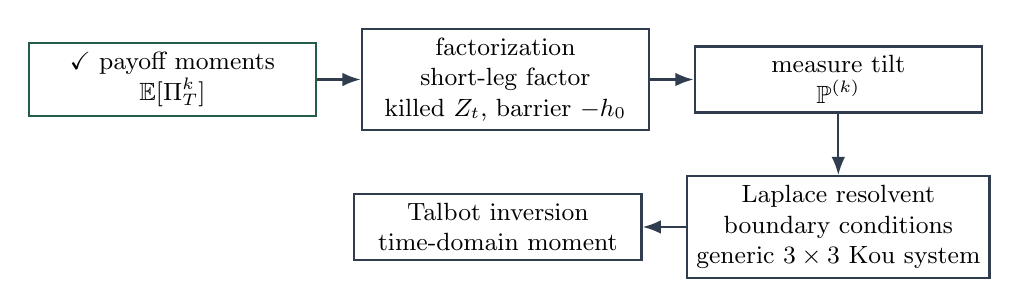
\begin{tikzpicture}[
      stage/.style={draw=slate,thick,minimum width=3.65cm,minimum height=0.82cm,align=center,font=\small},
      done/.style={draw=forest,thick,minimum width=3.65cm,minimum height=0.82cm,align=center,font=\small},
      arr/.style={-Latex,thick,slate}
    ]
      \node[done] (a) {$\checkmark$ payoff moments\\$\E[\Pi_T^k]$};
      \node[stage,right=0.55cm of a] (b) {factorization\\short-leg factor\\killed $Z_t$, barrier $-h_0$};
      \node[stage,right=0.55cm of b] (c) {measure tilt\\$\Pbb^{(k)}$};
      \node[stage,below=0.78cm of c] (d) {Laplace resolvent\\boundary conditions\\generic $3\times3$ Kou system};
      \node[stage,left=0.55cm of d] (e) {Talbot inversion\\time-domain moment};
      \draw[arr] (a) -- (b);
      \draw[arr] (b) -- (c);
      \draw[arr] (c) -- (d);
      \draw[arr] (d) -- (e);
    \end{tikzpicture}
  \end{center}
  \vspace{0.45em}
  Covered: payoff function + need for moments
  \vspace{0.25em}

  Next: factorization and measure change $\rightarrow$ one-dimensional killed expectation
  \[
    k\,\eta_{1,+}<1,\qquad k\,\eta_{2,+}<1
    \quad\text{moment-admissibility condition}
  \]
\end{frame}

% ------------------------------------------------------------
\begin{frame}{Factorization: From Two Assets to One Barrier}
  \small
  Motivation: separate terminal short-leg factor; isolate killed ratio problem
  \vspace{0.25em}

  Bivariate payoff; scalar liquidation state:
  \[
    Z_t=X_{1,t}-X_{2,t}
  \]
  Initial log health factor:
  \[
    h_0:=\log H_0
  \]
  Factorization using $H_T=e^{h_0+Z_T}$:
  \[
    \Pi_T
    =
    \frac{n_2}{b}\,S_{2,0}e^{X_{2,T}}
    (e^{h_0+Z_T}-b)\,\one_{\{\tau>T\}}
  \]
  One-dimensional payoff kernel:
  \[
    g_k(z;h_0):=(e^{h_0+z}-b)^k,
  \]
  Integer moments:
  \[
  \begin{aligned}
    \Pi_T^k
    &=
    \underbrace{
      \Big(\frac{n_2}{b}\Big)^kS_{2,0}^k e^{kX_{2,T}}
    }_{\mathcal F_T^{S_2}\text{ part}}
    \underbrace{
      g_k(Z_T;h_0)\,\one_{\{\tau>T\}}
    }_{\mathcal F_T^{Z}\text{ killed-ratio part}}
  \end{aligned}
  \]
  Measure change: absorb $\mathcal F_T^{S_2}$ factor; retain killed expectation under $Z$
  \vspace{0.3em}

  Barrier-option analogue: scalar state $Z$, barrier $-h_0$
\end{frame}

% ------------------------------------------------------------
\begin{frame}{Measure Change}
  \scriptsize
  Start from factorized moment:
  \[
    \E_\Pbb[\Pi_T^k]
    =
    \Big(\frac{n_2}{b}\Big)^kS_{2,0}^k\,
    \E_\Pbb\!\left[
      e^{kX_{2,T}}g_k(Z_T;h_0)\one_{\{\tau>T\}}
    \right]
  \]
  Exponential tilt:
  \[
    \left.\frac{d\Pbb^{(k)}}{d\Pbb}\right|_{\mathcal F_T}
    =
    \frac{e^{kX_{2,T}}}{\E[e^{kX_{2,T}}]}
  \]
  Heuristic reminder, with $Y=g_k(Z_T;h_0)\one_{\{\tau>T\}}$:
  \[
  \begin{aligned}
    \E_{\Pbb^{(k)}}[Y]
    &=
    \int Y\,d\Pbb^{(k)}
    =
    \int Y\,\frac{d\Pbb^{(k)}}{d\Pbb}\,d\Pbb\\
    &=
    \E_\Pbb\!\left[
      Y\,\frac{e^{kX_{2,T}}}{\E_\Pbb[e^{kX_{2,T}}]}
    \right]
    &=
    \frac{\E_\Pbb[e^{kX_{2,T}}Y]}{\E_\Pbb[e^{kX_{2,T}}]}
    \quad\Longrightarrow\quad
    \E_\Pbb[e^{kX_{2,T}}Y]
    =
    \E_\Pbb[e^{kX_{2,T}}]\E_{\Pbb^{(k)}}[Y]
  \end{aligned}
  \]
  {\scriptsize Remark: Radon--Nikodym theorem / change-of-measure identity}
  \vspace{0.15em}

  Reduced moment:
  \[
    \E[\Pi_T^k]
    =
    \Big(\frac{n_2}{b}\Big)^kS_{2,0}^k
    \E[e^{kX_{2,T}}]\,
    \E^{(k)}\!\left[
      g_k(Z_T;h_0)\one_{\{\tau>T\}}
    \right]
  \]
  Bivariate payoff moment $\rightarrow$ killed expectation of the ratio process
\end{frame}

% ------------------------------------------------------------
\begin{frame}{Tilted Ratio Process}
  \small
  Remaining object:
  \[
    \E^{(k)}\!\left[
      g_k(Z_T;h_0)\one_{\{\tau>T\}}
    \right]
  \]
  Question:
  \[
    Z_t=X_{1,t}-X_{2,t}
    \quad\text{under}\quad \Pbb^{(k)}
  \]
  Under $\Pbb^{(k)}$: $Z$ remains a L\'evy process

  L\'evy--Khintchine exponent of $Z$ under $\Pbb^{(k)}$:
  \[
    \psi_Z^{(k)}(s)
    =
    \mu_Z^{(k)}s+\frac12\sigma_Z^2s^2
    +\lambda_1\big(M_1(s)-1\big)
    +\lambda_2\big(M_2(k-s)-M_2(k)\big)
  \]
  with
  \[
    M_i(s)=
    \frac{p_i}{1-s\eta_{i,+}}
    +
    \frac{1-p_i}{1+s\eta_{i,-}},
    \qquad
    \sigma_Z^2=\sigma_1^2+\sigma_2^2-2\rho\sigma_1\sigma_2
  \]
  $\mathcal L^{(k)}$: infinitesimal generator of $Z$ under $\Pbb^{(k)}$, the generator eigenrelation:
  \[
    \mathcal L^{(k)}e^{sz}=\psi_Z^{(k)}(s)e^{sz}
  \]
\end{frame}

% ------------------------------------------------------------
\begin{frame}{Killed Moment PIDE}
  \small
  Target function:
  \[
    U(t,z)
    :=
    \E_z^{(k)}\!\left[
      g_k(Z_t;h_0)\one_{\{\tau(h_0)>t\}}
    \right],
    \qquad z>-h_0
  \]
  \vspace{0.2em}

  Backward Kolmogorov PIDE for the killed process:
  \[
    \partial_t U(t,z)=\mathcal L^{(k)}U(t,z),
    \qquad z>-h_0
  \]
  Initial and absorbing boundary:
  \[
    U(0,z)=g_k(z;h_0),
    \qquad
    U(t,z)=0\quad\text{for }z\le -h_0
  \]
  \vspace{0.2em}
  
  One time variable; one state variable $z$ for the ratio process $Z$

\end{frame}

% ------------------------------------------------------------
\begin{frame}{Laplace Transform Trick}
  \small
  Time-domain PIDE:
  \[
    \partial_t U(t,z)=\mathcal L^{(k)}U(t,z),
    \qquad
    U(0,z)=g_k(z;h_0)
  \]
  Laplace transform in time:
  \[
    \widehat U(q,z)=\int_0^\infty e^{-qt}U(t,z)\,dt,
    \qquad q>0
  \]
  Laplace-domain resolvent:
  \[
    (q-\mathcal L^{(k)})\widehat U(q,z)=g_k(z;h_0),
    \qquad z>-h_0
  \]
  Sepp~\cite{Sepp2004} idea:

  Laplace transform $+$ double-exponential jumps $\rightarrow$ finite algebraic system
  \vspace{0.25em}

  Here:
  \[
    \psi_Z^{(k)}(\gamma)=q
    \quad\Longrightarrow\quad
    \text{degree-six characteristic equation}
  \]
  Distinct downward phases: three admissible roots $+$ three boundary conditions
  $\rightarrow 3\times3$ system
\end{frame}

% ------------------------------------------------------------
\begin{frame}{Resolvent Solution Form}
  \small
  Resolvent decomposition:
  \[
    \widehat U(q,z;h_0)
    =
    \widehat U_{\mathrm{part}}(q,z;h_0)
    +
    \widehat U_{\mathrm{hom}}(q,z;h_0)
  \]
  Particular solution:
  \[
    \widehat U_{\mathrm{part}}(q,z;h_0)
    =
    \sum_{j=0}^{k}
    \frac{c_{k,j}(h_0)}{q-\psi_Z^{(k)}(j)}e^{jz}
  \]
  Homogeneous solution:
  \[
    \widehat U_{\mathrm{hom}}(q,z;h_0)
    =
    \sum_{m=1}^{3}
    B_m^{(k)}(q;h_0)e^{\gamma_{m+3}(q)(z+h_0)}
  \]
  Boundary coefficients:
  \[
    \underbrace{\mathbf M_{\mathrm{bar}}^{(k)}(q)}_{3\times3}
    \underbrace{\mathbf B^{(k)}}_{3\times1}
    =
    -\underbrace{\mathbf b^{(k)}}_{3\times1}
  \]
  PIDE solve $\rightarrow$ summation of exponentials $+$ one generic $3\times3$ linear system
\end{frame}

% ------------------------------------------------------------
\begin{frame}{Primary Output: Survival and Killed Moments}
  \small
  Objective-independent Laplace--resolvent outputs
  \vspace{0.4em}

  \begin{center}
  \begin{tabular}{rrrrrr}
    \toprule
    $h_0$ & $p_{\mathrm{surv}}$ & $M_1$ & $M_2$
    & $\E[\Pi_T\mid\tau>T]$ & $\E[\Pi_T^2\mid\tau>T]$ \\
    \midrule
    $0.0306$ & $0.356955$ & $0.646184$ & $1.268463$ & $1.810269$ & $3.553569$ \\
    $0.1000$ & $0.766735$ & $1.111927$ & $1.755024$ & $1.450210$ & $2.288957$ \\
    $0.2500$ & $0.989001$ & $1.214321$ & $1.606097$ & $1.227826$ & $1.623960$ \\
    $0.5000$ & $0.999995$ & $1.168318$ & $1.426096$ & $1.168324$ & $1.426104$ \\
    $1.0000$ & $1.000000$ & $1.132221$ & $1.314377$ & $1.132221$ & $1.314377$ \\
    $2.0000$ & $1.000000$ & $1.112544$ & $1.259450$ & $1.112544$ & $1.259450$ \\
    \bottomrule
  \end{tabular}
  \end{center}
  \vspace{0.5em}

  \footnotesize $M_k=p_{\mathrm{surv}}\E[\Pi_T^k\mid\tau>T]$; the first row is the
  protocol origination bound. Decision rules consume this map downstream.
\end{frame}

% ------------------------------------------------------------
\begin{frame}{Conditional Statistics and MC Survival}
  \scriptsize
  Secondary transformation of killed moments; Laplace--resolvent vs MC survival
  \vspace{0.15em}

  \begin{center}
  \resizebox{0.84\textwidth}{!}{%
  \begin{tabular}{cc cc cccc}
  \toprule
  $h_0$ & $H_0$ & $p_{\mathrm{surv}}^{\mathrm{Lap}}$ & $p_{\mathrm{surv}}^{\mathrm{MC}}$
  & Mean & Variance & Skewness & Ex.\ Kurt.\\
  \midrule
  $0.031$ & $1.031$ & $0.3570$ & $0.3751$ & $1.8103$ & $0.2765$ & $0.8541$ & $1.0512$ \\
  $0.10$ & $1.105$ & $0.7667$ & $0.7748$ & $1.4502$ & $0.1858$ & $0.7909$ & $0.8748$ \\
  $0.25$ & $1.284$ & $0.9890$ & $0.9893$ & $1.2278$ & $0.1164$ & $0.5294$ & $0.4890$ \\
  $0.50$ & $1.649$ & $1.0000$ & $1.0000$ & $1.1683$ & $0.0611$ & $0.4895$ & $0.5392$ \\
  $0.75$ & $2.117$ & $1.0000$ & $1.0000$ & $1.1451$ & $0.0414$ & $0.5120$ & $0.5510$ \\
  $1.00$ & $2.718$ & $1.0000$ & $1.0000$ & $1.1322$ & $0.0325$ & $0.5183$ & $0.5486$ \\
  $1.50$ & $4.482$ & $1.0000$ & $1.0000$ & $1.1189$ & $0.0248$ & $0.5132$ & $0.5297$ \\
  $2.00$ & $7.389$ & $1.0000$ & $1.0000$ & $1.1125$ & $0.0217$ & $0.5041$ & $0.5109$ \\
  \midrule
  $\infty$ & $\infty$ & $1.0000$ & --- & $1.1046$ & $0.0183$ & $0.4845$ & $0.4747$ \\
  \bottomrule
  \end{tabular}}
  \end{center}
  \vspace{0.2em}

  \begin{itemize}
    \item Smaller $H_0$: lower survival probability; higher liquidation probability
    \item Conditional mean declines toward the long-WETH no-shorting limit; survivor selection amplifies it near the barrier
    \item Conditional variance: decreasing as $H_0$ increases
  \end{itemize}
  \vspace{0.1em}

  Bottom row: no-shorting analytical limit
\end{frame}

% ------------------------------------------------------------
\begin{frame}{Numerical Example}
  \scriptsize
  Laplace minus MC; wall-clock computation time
  \vspace{0.15em}

  \begin{center}
  \resizebox{0.84\textwidth}{!}{%
  \begin{tabular}{cc rrrrr rr}
  \toprule
  $h_0$ & $H_0$ & $\Delta p_{\mathrm{surv}}$ & $\Delta$Mean
  & $\Delta$Var. & $\Delta$Skew. & $\Delta$Kurt.
  & Lap. & MC \\
  \midrule
  $0.031$ & $1.031$ & $-0.0181$ & $\phantom{-}0.0111$ & $\phantom{-}0.0039$ & $\phantom{-}0.0188$ & $\phantom{-}0.0505$ & $0.069$ & $51.09$ \\
  $0.10$ & $1.105$ & $-0.0080$ & $\phantom{-}0.0045$ & $\phantom{-}0.0011$ & $\phantom{-}0.0257$ & $\phantom{-}0.0717$ & $0.067$ & $49.51$ \\
  $0.25$ & $1.284$ & $-0.0002$ & $\phantom{-}0.0005$ & $\phantom{-}0.0004$ & $\phantom{-}0.0237$ & $\phantom{-}0.0503$ & $0.067$ & $49.62$ \\
  $0.50$ & $1.649$ & $\phantom{-}0.0000$ & $\phantom{-}0.0003$ & $\phantom{-}0.0002$ & $\phantom{-}0.0189$ & $\phantom{-}0.0445$ & $0.067$ & $49.42$ \\
  $0.75$ & $2.117$ & $\phantom{-}0.0000$ & $\phantom{-}0.0002$ & $\phantom{-}0.0001$ & $\phantom{-}0.0168$ & $\phantom{-}0.0397$ & $0.067$ & $49.61$ \\
  $1.00$ & $2.718$ & $\phantom{-}0.0000$ & $\phantom{-}0.0002$ & $\phantom{-}0.0000$ & $\phantom{-}0.0147$ & $\phantom{-}0.0343$ & $0.067$ & $49.51$ \\
  $1.50$ & $4.482$ & $\phantom{-}0.0000$ & $\phantom{-}0.0002$ & $\phantom{-}0.0000$ & $\phantom{-}0.0114$ & $\phantom{-}0.0250$ & $0.068$ & $49.83$ \\
  $2.00$ & $7.389$ & $\phantom{-}0.0000$ & $\phantom{-}0.0002$ & $\phantom{-}0.0000$ & $\phantom{-}0.0094$ & $\phantom{-}0.0187$ & $0.068$ & $50.41$ \\
  \bottomrule
  \end{tabular}}
  \end{center}
  \vspace{0.2em}

  \begin{itemize}
    \item $\Delta p_{\mathrm{surv}}<0$: MC misses intra-period barrier crossings
    \item Gap largest near $H_0^{\min}$; negligible for larger health buffers
    \item Host-specific runtime: Laplace $\approx0.07$s vs grid-monitored MC $\approx49$--$51$s
  \end{itemize}
\end{frame}

% ------------------------------------------------------------
\begin{frame}{Application: Objective-Specific Sizing}
  Choice variable: $h_0=\log H_0$; equivalently initial borrow amount
  \vspace{0.3em}

  One illustrative objective:
  \[
  \begin{aligned}
    \Phi(h_0)
    &=
    \E[\Pi_T\mid \tau>T]
    -\frac{\alpha}{2}\operatorname{Var}(\Pi_T\mid \tau>T)
    -\delta\,\liq(h_0),
  \end{aligned}
  \]
  Liquidation probability:
  \[
    \liq(h_0)=\Pbb(\tau\leq T)
  \]
  Objective-specific selection:
  \[
    h_0^\star\in\arg\max_{h_0\in\mathcal H(b,\ell_{\max})}\Phi(h_0)
  \]
  Alternatives use the same evaluation map: a liquidation constraint or unconditional
  killed-payoff mean--variance. No rule is designated as universally correct.
\end{frame}

% ------------------------------------------------------------
\begin{frame}{Same Engine, Different Selections}
  \scriptsize
  Baseline calibration; 200-point grid on $H_0\in[1.031,2.000]$
  \vspace{0.3em}

  \begin{center}
    \begin{tabular}{llrrr}
      \toprule
      Rule & Parameters & Selected $H_0$ & $L_0$ & $p_{\mathrm{liq}}$ \\
      \midrule
      Max.\ leverage under cap & $\bar p=0.05$ & $1.201$ & $3.234$ & $0.0494$ \\
      Max.\ leverage under cap & $\bar p=0.10$ & $1.163$ & $3.496$ & $0.0954$ \\
      Max.\ leverage under cap & $\bar p=0.20$ & $1.119$ & $3.875$ & $0.1905$ \\
      Unconditional killed MV & $\alpha=1$ & $1.338$ & $2.634$ & $0.0039$ \\
      Conditional MV $+$ penalty & $(\alpha,\delta)=(1,0)$ & $1.031^\dagger$ & $5.128$ & $0.6430$ \\
      Conditional MV $+$ penalty & $(\alpha,\delta)=(1,0.5)$ & $1.031^\dagger$ & $5.128$ & $0.6430$ \\
      \bottomrule
    \end{tabular}
  \end{center}
  \vspace{0.35em}

  $^\dagger$Candidate-grid endpoint. The selected buffer changes with the rule and
  preference parameters; no row is a universal recommendation.
\end{frame}

% ------------------------------------------------------------
\begin{frame}{Sampling Uncertainty Is Material}
  \small
  Paired circular moving-block bootstrap: 40 recalibrations, 1.5-day blocks,
  90\% percentile intervals. Downstream rule: maximize $L_0$ subject to
  $p_{\mathrm{liq}}\leq0.10$ on the same 200-point grid.
  \vspace{0.6em}

  \begin{center}
    \begin{tabular}{lrr}
      \toprule
      Quantity & Point & 90\% interval \\
      \midrule
      $p_{\mathrm{surv}}$ at $H_0=1.163$ & $0.905$ & $[0.501,0.976]$ \\
      Selected $H_0$ & $1.163$ & $[1.108,1.362]$ \\
      Selected $L_0$ & $3.496$ & $[2.559,3.981]$ \\
      \bottomrule
    \end{tabular}
  \end{center}
  \vspace{0.6em}

  \footnotesize Conditional on the Kou model, ECF criterion, preprocessing,
  protocol terms, block length, and sizing grid; not a model-selection or
  out-of-sample forecast interval.
\end{frame}

% ------------------------------------------------------------
\begin{frame}[plain]
  \begin{tikzpicture}[remember picture,overlay]
    \node at (current page.center) {%
    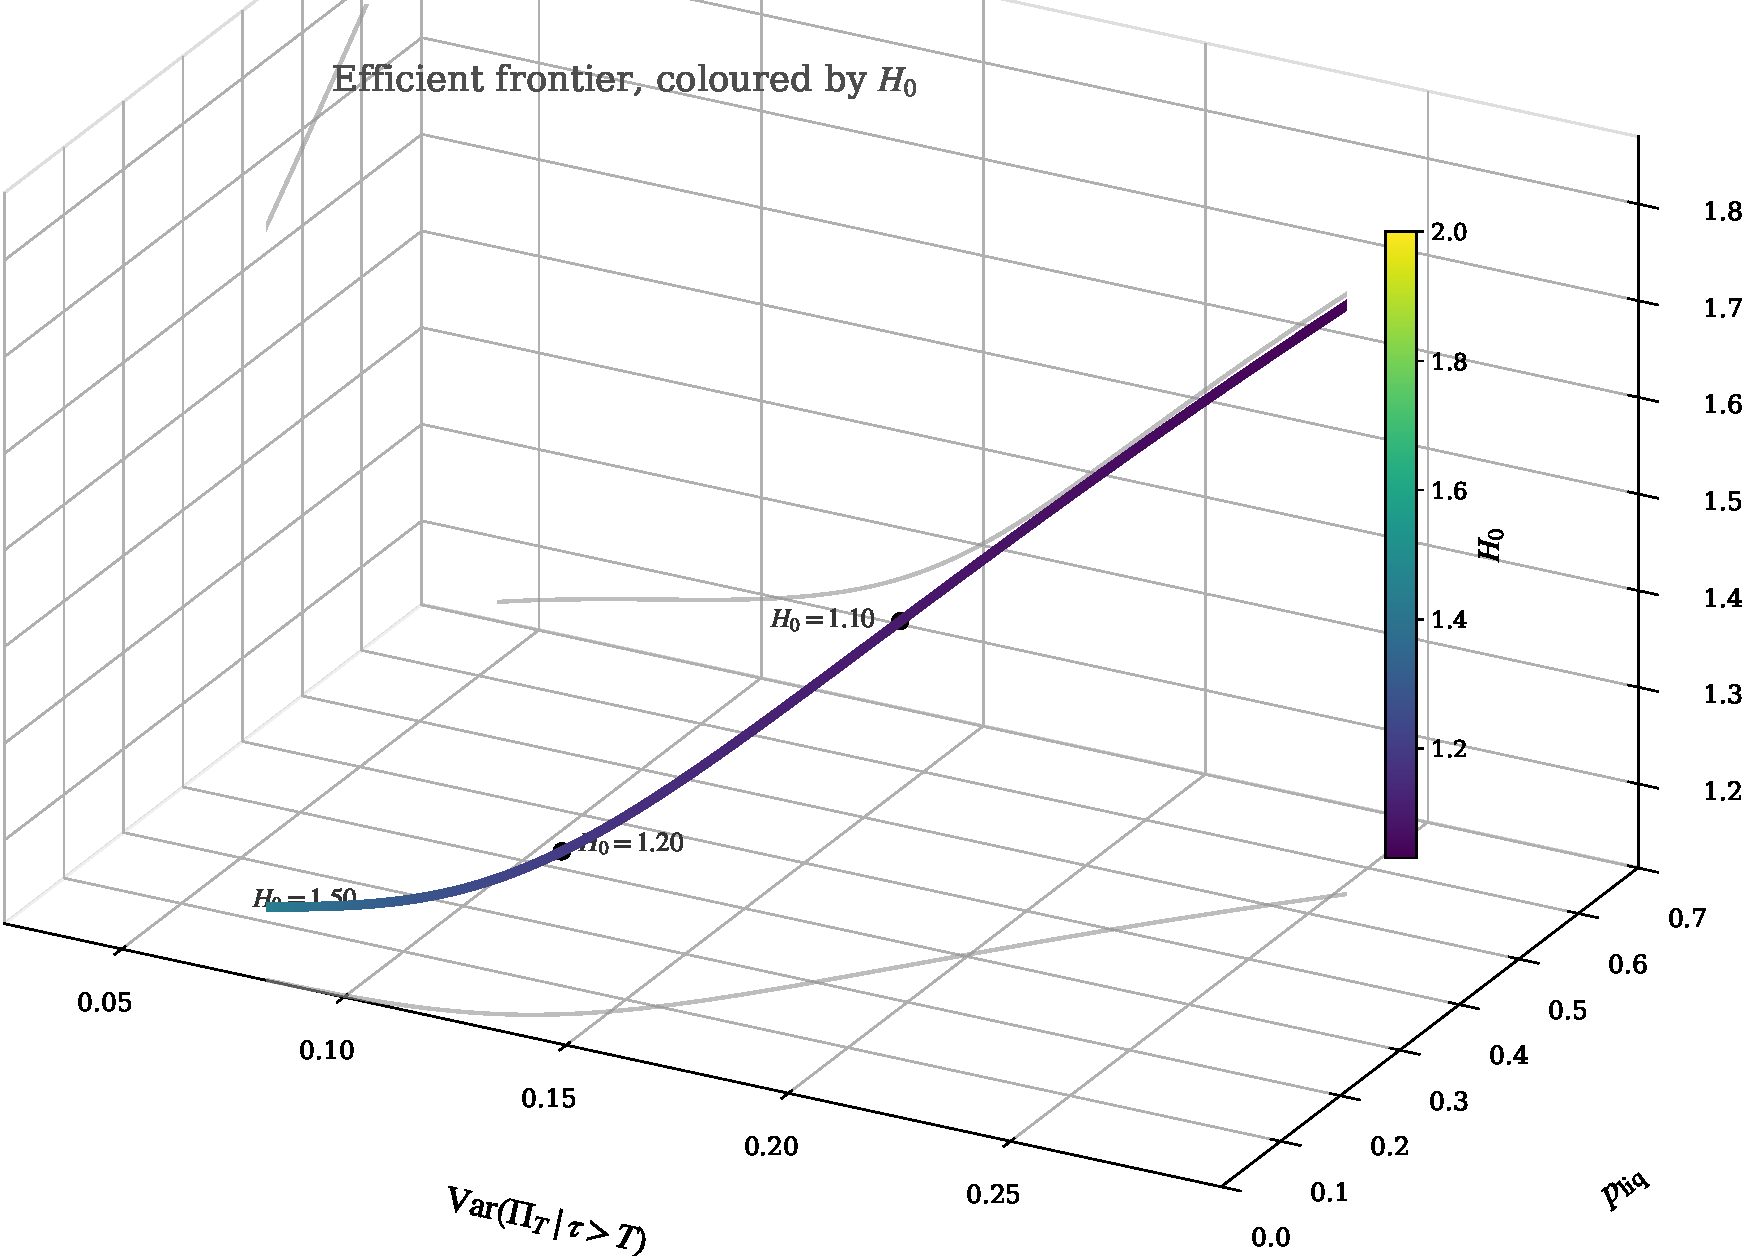
\includegraphics[width=1.06\paperwidth,height=0.98\paperheight,keepaspectratio]{fig_frontier_3d.pdf}%
    };
  \end{tikzpicture}
\end{frame}

% ------------------------------------------------------------
\begin{frame}{Conclusions and Discussion}
  \begin{itemize}
    \item DeFi long--short $\rightarrow$ collateral/debt first passage
    \item Measure change $\rightarrow$ one-dimensional killed expectations of $Z=X_1-X_2$
    \item Kou jump diffusion $\rightarrow$ finite-dimensional Laplace resolvent
    \item Primary output: $h_0\mapsto$ survival and killed-payoff moment characteristics
    \item Sizing is an objective-specific application of that map
  \end{itemize}
  \vspace{0.8em}
  \textbf{Scope limits}
  \begin{itemize}
    \item Killed-payoff benchmark does not model liquidation recovery
    \item Static buffer only: no collateral intervention, oracle/keeper delay, or execution cost
    \item Selected buffers remain objective-, model-, and calibration-dependent
  \end{itemize}
  \vfill
  \begin{center}
    \large Thank you
  \end{center}
\end{frame}

% ------------------------------------------------------------
\begin{frame}{References}
  \footnotesize
  \bibliographystyle{abbrvnat}
  \bibliography{finance}
\end{frame}

\end{document}
